\documentclass[10pt,letterpaper,oneside]{article}
\usepackage[T1]{fontenc}
\usepackage[utf8]{inputenc}
\usepackage{lmodern}
\usepackage[scaled=0.93]{inconsolata}
\usepackage[margin=0.79in,headheight=16pt,headsep=15pt,footskip=27pt]{geometry}
\usepackage{microtype}
\usepackage{amssymb}
\usepackage{xcolor}
\usepackage{graphicx}
\usepackage{tikz}
\usepackage{array,booktabs,longtable,tabularx,multirow}
\usepackage{enumitem}
\usepackage{titlesec}
\usepackage{fancyhdr,lastpage}
\usepackage[most]{tcolorbox}
\usepackage{listings}
\usepackage{hyperref,xurl}
\usepackage{needspace}
\usetikzlibrary{arrows.meta,positioning,shapes.geometric,calc}
\definecolor{navy}{HTML}{10233D}
\definecolor{blue}{HTML}{1763A0}
\definecolor{teal}{HTML}{087D82}
\definecolor{pale}{HTML}{EDF5F8}
\definecolor{graytext}{HTML}{465465}
\definecolor{linegray}{HTML}{CED9E3}
\definecolor{codebg}{HTML}{F4F7FA}
\definecolor{orange}{HTML}{A85F19}
\definecolor{softorange}{HTML}{FFF5E9}
\definecolor{forest}{HTML}{25634A}
\hypersetup{hypertexnames=false,colorlinks=true,linkcolor=blue,urlcolor=blue,citecolor=blue,pdftitle={HTTP Request Metadata: Cross-Platform Engineering and Security Guide},pdfauthor={Technical Reference},pdfsubject={HTTP URL parsing, request metadata, reverse proxies, application security}}
\urlstyle{same}
\setlength{\parindent}{0pt}
\setlength{\parskip}{5pt plus 1pt}
\setlist[itemize]{topsep=3pt,itemsep=2pt,leftmargin=1.45em}
\setlist[enumerate]{topsep=3pt,itemsep=3pt,leftmargin=1.55em}
\renewcommand{\arraystretch}{1.17}
\titleformat{\section}{\Large\bfseries\color{navy}}{\thesection}{0.65em}{}[\vspace{-3pt}\color{linegray}\titlerule]
\titleformat{\subsection}{\large\bfseries\color{blue}}{\thesubsection}{0.55em}{}
\titleformat{\subsubsection}{\normalsize\bfseries\color{navy}}{\thesubsubsection}{0.5em}{}
\titlespacing*{\section}{0pt}{19pt}{9pt}
\titlespacing*{\subsection}{0pt}{13pt}{5pt}
\pagestyle{fancy}
\fancyhf{}
\fancyhead[L]{\footnotesize\color{graytext}\textsf{HTTP REQUEST METADATA}}
\fancyhead[R]{\footnotesize\color{graytext}\textsf{ENGINEERING / APPSEC REFERENCE}}
\fancyfoot[L]{\footnotesize\color{graytext}11 October 2026 \quad|\quad Version 1.0}
\fancyfoot[R]{\footnotesize\color{graytext}Page \thepage\ of \pageref{LastPage}}
\renewcommand{\headrulewidth}{0.3pt}
\renewcommand{\footrulewidth}{0pt}
\newcolumntype{Y}{>{\raggedright\arraybackslash}X}
\newcolumntype{P}[1]{>{\raggedright\arraybackslash}p{#1}}
\newtcolorbox{keybox}[1][]{enhanced,breakable,colback=pale,colframe=teal,boxrule=0.7pt,arc=2mm,left=11pt,right=11pt,top=8pt,bottom=8pt,#1}
\newtcolorbox{riskbox}[1][]{enhanced,breakable,colback=softorange,colframe=orange,boxrule=0.6pt,arc=2mm,left=11pt,right=11pt,top=8pt,bottom=8pt,#1}
\newcommand{\term}[1]{\textbf{\texttt{#1}}}
\newcommand{\nil}{\textit{none / not universal}}
\newcommand{\refs}[1]{\textsuperscript{\color{blue}[#1]}}
\lstdefinelanguage{JavaScript}{morekeywords={const,let,var,function,return,if,else,async,await,new,true,false,null,require},sensitive=true,morecomment=[l]{//},morecomment=[s]{/*}{*/},morestring=[b]" ,morestring=[b]'}
\lstdefinelanguage{bash}{morekeywords={curl,echo,export,python,go,php,node},sensitive=true,morecomment=[l]{\#},morestring=[b]" ,morestring=[b]'}
\lstdefinelanguage{GoLang}{morekeywords={package,import,func,var,const,return,if,else,for,range,struct,map,string,bool,byte,error,nil,true,false,defer,go,type},sensitive=true,morecomment=[l]{//},morecomment=[s]{/*}{*/},morestring=[b]"}
\lstdefinelanguage{CSharpLite}{morekeywords={using,var,new,string,object,public,class,static,void,async,await,return,if,else,true,false,null,namespace,record},sensitive=true,morecomment=[l]{//},morecomment=[s]{/*}{*/},morestring=[b]"}
\lstdefinelanguage{Plain}{morekeywords={},sensitive=true}
\lstset{basicstyle=\ttfamily\footnotesize,backgroundcolor=\color{codebg},frame=single,rulecolor=\color{linegray},framesep=7pt,breaklines=true,breakatwhitespace=false,columns=fullflexible,keepspaces=true,showstringspaces=false,tabsize=2,upquote=true,keywordstyle=\color{blue}\bfseries,commentstyle=\color{forest}\itshape,stringstyle=\color{orange},aboveskip=8pt,belowskip=9pt}
\newcommand{\code}[1]{\texttt{#1}}
\begin{document}
\begin{titlepage}
\thispagestyle{empty}
\vspace*{1.05in}
{\sffamily\bfseries\color{teal}\fontsize{13}{16}\selectfont ENGINEERING REFERENCE SERIES}\par
\vspace{0.28in}
{\sffamily\bfseries\color{navy}\fontsize{31}{38}\selectfont HTTP REQUEST\\[4pt]METADATA}\par
\vspace{0.12in}
{\sffamily\color{blue}\fontsize{17}{24}\selectfont Cross-Platform Engineering \& Security Guide}\par
\vspace{0.35in}
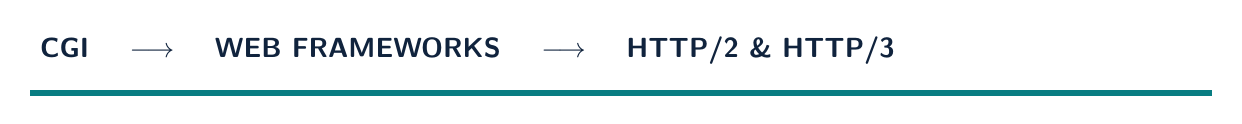
\begin{tikzpicture}
\draw[teal,line width=2pt] (0,0)--(15.0,0);
\node[anchor=west,font=\sffamily\bfseries\color{navy}] at (0,0.54) {CGI \quad $\longrightarrow$ \quad WEB FRAMEWORKS \quad $\longrightarrow$ \quad HTTP/2 \& HTTP/3};
\end{tikzpicture}
\vspace{0.37in}
{\large\color{graytext}Java Servlet / Jakarta EE \quad\textbullet\quad ASP.NET Core \quad\textbullet\quad PHP\\
Python (WSGI / ASGI) \quad\textbullet\quad Node.js / Express \quad\textbullet\quad Go}\par
\vfill
\begin{tcolorbox}[colback=pale,colframe=linegray,boxrule=0.5pt,arc=1.5mm,left=13pt,right=13pt,top=12pt,bottom=12pt]
\textbf{In this guide}\par
URI anatomy \textbullet\ legacy variable crosswalk \textbullet\ raw vs. decoded values \textbullet\ copyable diagnostics \textbullet\ proxy trust boundaries \textbullet\ exploit classes \textbullet\ verification matrix \textbullet\ primary specifications
\end{tcolorbox}
\vspace{0.27in}
{\small\textbf{Edition:} 1.0 \qquad \textbf{Issued:} 11 October 2026 \qquad \textbf{Audience:} Backend / platform / AppSec engineers}\par
{\footnotesize\color{graytext}Technical synthesis based on publicly documented protocol specifications and framework APIs. The diagnostics in this guide are intended for controlled development environments, not public production exposure.}
\end{titlepage}
\pagenumbering{roman}
\tableofcontents
\clearpage
\section*{Executive reference card}
\addcontentsline{toc}{section}{Executive reference card}
\begin{keybox}
\textbf{Five invariants to remember}
\begin{enumerate}
\item \textbf{URI components are not all headers.} The request target supplies the path/query; authority comes from \code{Host} or \code{:authority} in applicable protocol versions.
\item \textbf{Raw, percent-encoded, decoded, normalized, and routed paths are different views.} Do not substitute one for another without an explicit rule.
\item \textbf{\code{PATH\_TRANSLATED} is not a route, and it is not always present.} It is legacy web-server-dependent filesystem translation. Never use it as an authorization primitive.
\item \textbf{Proxy metadata is a separate trust boundary.} \code{Forwarded} and \code{X-Forwarded-*} are untrusted unless processed under a specific, enforceable trusted-proxy policy.
\item \textbf{Build public URLs from configured origins, not arbitrary input.} Treat request authority, forwarded host, paths, and query values as hostile until validated.
\end{enumerate}
\end{keybox}
\begin{table}[h!]
\centering\small
\begin{tabularx}{\linewidth}{P{0.27\linewidth}Y}
\toprule
\textbf{You need to know\ldots} & \textbf{Use / verify\ldots}\\\midrule
Exact incoming request target & Server/container raw request-target interface, if offered; intermediaries may have rewritten it.\\
Application path & Framework path after mount/rewrite/decoding; document normalization behavior.\\
Route parameters & Router binding, not path string splitting; validate type and authorization.\\
Query parameters & Framework parser for ordinary values; raw query when signature/canonicalization requires byte fidelity.\\
Client-facing scheme/host & Trusted proxy configuration and an explicit external-origin allowlist.\\
Client IP & Network peer address or vetted forwarded chain; define an auditable trust policy.\\
File to serve & Fixed storage root, safe path resolution, and strict containment check; never legacy translation alone.\\
\bottomrule
\end{tabularx}
\end{table}
\begin{riskbox}
\textbf{Important scope limit.} APIs expose observations from their current processing layer, \emph{not necessarily the bytes sent by the original client}. A CDN, ingress, proxy, web server, framework, or router may have decoded or rewritten the request earlier. The example code reports request metadata for teaching and local verification; remove it or strictly protect it before production release.
\end{riskbox}
\clearpage
\pagenumbering{arabic}
\section{Conceptual and protocol foundation}
\subsection{Decomposing a target URI}
\begin{lstlisting}[language=Plain]
https://api.example.test:8443/gateway/v1/orders/42?view=full&tag=a&tag=b#details
\___/   \______________/ \___________________/ \____________________/ \_____/
 scheme       authority           path               query         fragment
\end{lstlisting}
The fragment (\code{\#details}) is handled by the client and is \emph{not} part of the HTTP target URI sent to the origin. A typical HTTP/1.1 origin request contains the request target \code{/gateway/v1/orders/42?view=full\&tag=a\&tag=b}, plus \code{Host: api.example.test:8443}. The \code{?} divides path and query; a \code{?} or \code{/} that is percent-encoded within a component is data until interpreted by a component-aware parser. RFC 3986 defines the generic URI grammar, while RFC 9110 defines HTTP semantics.\refs{1,2}

\begin{figure}[h!]
\centering
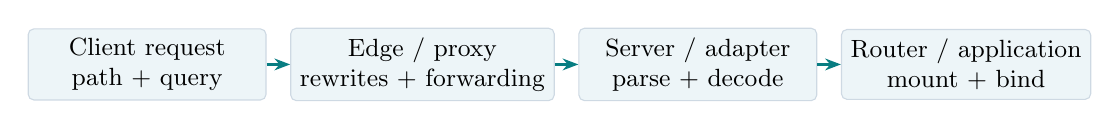
\begin{tikzpicture}[font=\small, node distance=3mm]
\tikzset{phase/.style={draw=linegray,rounded corners=2pt,fill=pale,align=center,minimum width=3.02cm,minimum height=0.78cm}}
\node[phase] (wire) {Client request\\path + query};
\node[phase,right=of wire] (edge) {Edge / proxy\\rewrites + forwarding};
\node[phase,right=of edge] (server) {Server / adapter\\parse + decode};
\node[phase,right=of server] (app) {Router / application\\mount + bind};
\draw[-{Stealth[length=2mm]},thick,teal] (wire)--(edge);
\draw[-{Stealth[length=2mm]},thick,teal] (edge)--(server);
\draw[-{Stealth[length=2mm]},thick,teal] (server)--(app);
\end{tikzpicture}
\caption{Processing stages can change the representation or meaning of request metadata.}
\end{figure}

\subsection{Transport conventions across HTTP versions}
\begin{tabularx}{\linewidth}{P{0.19\linewidth}Y Y}
\toprule
\textbf{Aspect} & \textbf{HTTP/1.1} & \textbf{HTTP/2 and HTTP/3}\\\midrule
Target representation & Request line: \code{GET /p?x=1 HTTP/1.1} & Pseudo-headers such as \code{:method}, \code{:scheme}, \code{:authority}, \code{:path}\\
Authority & \code{Host} is mandatory on requests & Usually \code{:authority}; consistency with \code{Host} must be enforced as applicable\\
Path + query & Origin-form request target (most common) & \code{:path} normally includes path plus optional \code{?query}\\
App-level exposure & Parsed by HTTP server/framework & Typically translated into essentially the same framework request abstraction\\
Special forms & Absolute-form, authority-form for \code{CONNECT}, asterisk-form for \code{OPTIONS} & Method-specific CONNECT rules / special handling; do not assume every request has an ordinary path\\
\bottomrule
\end{tabularx}
\par
The four HTTP/1.1 request-target forms are specified in RFC 9112; HTTP/2 and HTTP/3 pseudo-header requirements are defined in RFCs 9113 and 9114. Most applications should use their framework abstraction and reserve raw protocol parsing for infrastructure components.\refs{2,3,4,5}

\subsection{Four distinct path representations}
\begin{tabularx}{\linewidth}{P{0.24\linewidth}Y}
\toprule
\textbf{Representation} & \textbf{Meaning and diagnostic use}\\\midrule
Raw encoded target & Observed request-target, often path plus raw query; can retain percent-encoding and parameter order.\\
Decoded path & A text representation; reserved characters such as encoded slashes can change segment boundaries if decoded incorrectly.\\
Mounted / routed path & Application-relative path after the container, mounting, rewriting, or routing; often paired with route values.\\
Filesystem translation & A server-dependent resolved physical path for a legacy script-oriented deployment; \emph{not} a general HTTP path concept.\\
\bottomrule
\end{tabularx}

\section{Legacy CGI variables: corrected interpretations}
RFC 3875 documents the traditional CGI meta-variables. They remain valuable historical terminology, especially for PHP and WSGI, but do not establish a uniform modern framework API.\refs{6}
\begin{longtable}{P{0.19\linewidth}P{0.40\linewidth}P{0.32\linewidth}}
\toprule
\textbf{Variable} & \textbf{Precise CGI-oriented meaning} & \textbf{Modern caution}\\\midrule\endfirsthead
\toprule\textbf{Variable} & \textbf{Precise CGI-oriented meaning} & \textbf{Modern caution}\\\midrule\endhead
\code{PATH\_INFO} & Extra logical path segment associated with a script/handler beyond \code{SCRIPT\_NAME}. & Not always defined; modern router paths are not necessarily equivalent.\\
\code{PATH\_TRANSLATED} & Server-dependent virtual-to-physical mapping of \code{PATH\_INFO}, performed as a separate local URI translation. & Often absent / \code{null}; must not be interpreted as an authenticated or sandboxed filesystem location.\\
\code{QUERY\_STRING} & Raw encoded query portion following the question mark, excluding the question mark. & May be empty or absent; parsing may collapse duplicates or alter encoding/order.\\
\code{SCRIPT\_NAME} & Virtual URI path identifying the running script or script mount. & Modern frameworks often do not execute a distinct script for each URL.\\
\code{REQUEST\_METHOD} & HTTP request method token. & Routing may expose or override effective method; check actual method and policy.\\
\code{SERVER\_PROTOCOL} & Protocol version string, typically at the CGI/web-server boundary. & May describe only the proxy-to-origin hop.\\
\code{HTTP\_HOST} / \code{SERVER\_NAME} & Request authority header / configured server identifier in applicable environments. & Host-derived values are user-influenced and require validation.\\
\code{REMOTE\_ADDR} & Connecting peer's address at the receiving server. & Behind proxies, normally describes the nearest upstream peer.\\
\bottomrule
\end{longtable}
\begin{riskbox}
\textbf{Correction to the legacy image's generalization:} \code{PATH\_TRANSLATED} does not mean ``a filename mapped to the real file system'' for every request or stack; it is specifically derived from \code{PATH\_INFO} under implementation-dependent CGI translation. Likewise, the Java Servlet API does \emph{not} define \code{getServerPath()}; use \code{getServletPath()} and \code{getContextPath()} for different pieces of servlet routing. ASP.NET Core does not preserve the legacy \code{Request.ServerVariables(...)} API.\refs{6,7,8}
\end{riskbox}

\section{Comparative API crosswalk}
\small
\begin{longtable}{P{0.16\linewidth}P{0.20\linewidth}P{0.22\linewidth}P{0.31\linewidth}}
\toprule
\textbf{Stack} & \textbf{Path and raw target} & \textbf{Query} & \textbf{Mount / script / special notes}\\\midrule\endfirsthead
\toprule\textbf{Stack} & \textbf{Path and raw target} & \textbf{Query} & \textbf{Mount / script / special notes}\\\midrule\endhead
Jakarta Servlet 6.1 & \code{getRequestURI()}, \code{getPathInfo()}, \code{getServletPath()} & \code{getQueryString()}, \code{getParameter*()} & \code{getContextPath()}; \code{getPathTranslated()} can return \code{null}. Request URI omits query.\\
ASP.NET Core & \code{Request.Path}, \code{Request.PathBase} & \code{Request.QueryString}, \code{Request.Query} & \code{Request.RouteValues}; no portable \code{PATH\_TRANSLATED}; \code{Path} is partially decoded (encoded \code{/} preserved).\\
PHP & \code{\$\_SERVER['REQUEST\_URI']}, optional \code{PATH\_INFO} & \code{\$\_SERVER['QUERY\_STRING']}, \code{\$\_GET} & \code{SCRIPT\_NAME}, \code{SCRIPT\_FILENAME}, \code{PATH\_TRANSLATED} vary by SAPI/server.\\
Python WSGI & \code{environ['PATH\_INFO']} & \code{environ['QUERY\_STRING']} & \code{SCRIPT\_NAME} mount prefix, \code{wsgi.url\_scheme}; CGI-compatible interface.\\
Python ASGI & \code{scope['path']}, optional \code{scope['raw\_path']} & \code{scope['query\_string']} (bytes) & \code{scope['root\_path']} mount prefix; \code{path} is decoded Unicode text.\\
Node.js core & \code{req.url} (target), \code{new URL(...).pathname} & \code{URLSearchParams} & \code{req.url} includes query; no built-in CGI script/mount semantics.\\
Express 5 & \code{req.originalUrl}, \code{req.url}, \code{req.path} & \code{req.query} & \code{req.baseUrl} in mounted middleware; \code{req.params} for route captures.\\
Go \code{net/http} & \code{r.RequestURI}, \code{r.URL.Path}, \code{r.URL.EscapedPath()} & \code{r.URL.RawQuery}, \code{r.URL.Query()} & \code{r.URL.RawPath} is optional hint, not a guaranteed raw-path mirror; no general CGI mount field.\\
\bottomrule
\end{longtable}
\normalsize
\textbf{Interpretation rule:} The table maps \emph{concepts}, not necessarily byte-identical values. Even within one language, deployment topology, router, middleware, and server configuration can alter which view is returned.\refs{7,8,9,10,11,12,13,14}

\section{A worked example: preserve the boundaries}
Assume the external URL is:
\begin{lstlisting}[language=Plain]
https://shop.example.test/store/api/items/42?tag=red&tag=blue&next=%2Fcart
\end{lstlisting}
A trusted reverse proxy removes the \code{/store} prefix before forwarding to a service at \path{http://10.2.0.7:8080/api/items/42?...}. The application's incoming connection sees \code{10.2.0.1} as its peer.

\smallskip
\noindent\begin{tabularx}{\linewidth}{P{0.31\linewidth}Y}
\toprule\textbf{Metadata view} & \textbf{Possible value}\\\midrule
Public scheme/authority & \code{https://shop.example.test}\\
External path & \code{/store/api/items/42}\\
Internal path & \code{/api/items/42}\\
External mount prefix & \code{/store} \emph{only if communicated/configured correctly}\\
Raw query & {\footnotesize\ttfamily tag=red\&tag=blue\&next=\%2Fcart}\\
Parsed query & \code{tag = [red, blue]}, \code{next = /cart} \emph{if parser retains repeats}\\
Transport peer & \code{10.2.0.1} (proxy)\\
Claimed original client & A forwarded chain; \emph{not inherently trustworthy}\\
\bottomrule
\end{tabularx}

No universal CGI variable reconstructs these facts. A safe design selects the authoritative source of each attribute, configures the public origin separately, and tests the exact ingress behavior.

\section{Java: Jakarta Servlet / Jakarta EE}
\subsection{Modern servlet APIs}
The \code{jakarta.servlet.http.HttpServletRequest} API is the successor to the \code{javax.servlet} namespace found in older Java EE applications. Servlet 6.1 documents \code{getPathInfo()}, \code{getPathTranslated()}, \code{getRequestURI()}, \code{getServletPath()}, \code{getContextPath()}, and \code{getQueryString()}. In normal configurations, path-info is canonicalized and suspicious sequences may be rejected by the container; \code{getRequestURI()} is a different representation and does not include the query.\refs{7}
\begin{lstlisting}[language=Java,caption={Jakarta Servlet diagnostic endpoint (development only)}]
import jakarta.servlet.annotation.WebServlet;
import jakarta.servlet.http.HttpServlet;
import jakarta.servlet.http.HttpServletRequest;
import jakarta.servlet.http.HttpServletResponse;
import java.io.IOException;

@WebServlet("/inspect/*")
public final class MetadataServlet extends HttpServlet {
    @Override
    protected void doGet(HttpServletRequest req,
                         HttpServletResponse resp) throws IOException {
        resp.setContentType("text/plain;charset=UTF-8");
        resp.getWriter().printf(
            "method=%s%ncontextPath=%s%nservletPath=%s%n" +
            "pathInfo=%s%npathTranslated=%s%nrequestURI=%s%n" +
            "queryString=%s%nremoteAddr=%s%n",
            req.getMethod(), req.getContextPath(),
            req.getServletPath(), req.getPathInfo(),
            req.getPathTranslated(), req.getRequestURI(),
            req.getQueryString(), req.getRemoteAddr()
        );
    }
}
\end{lstlisting}
For \code{/app/inspect/a/b?x=1}, deployed with context \code{/app} and mapping \code{/inspect/*}, typical values are \code{contextPath=/app}, \code{servletPath=/inspect}, \code{pathInfo=/a/b}, and \code{queryString=x=1}. This mapping-dependent illustration is not universal for exact, default, or extension servlet mappings. Do not treat \code{getPathTranslated()} as a safe file authorization decision.

\subsection{Java implementation notes}
\begin{itemize}
\item \code{getRequestURI()} is the request URI path component, excluding query. \code{getQueryString()} supplies the query separately.
\item \code{getParameterValues("tag")} is preferable to \code{getParameter("tag")} when repeated parameters matter; parameter parsing may include form-body inputs in addition to query inputs.
\item \code{getHttpServletMapping()} can help describe the actual matched servlet mapping; \code{getServletPath()} is not always a CGI-style script file name.
\item A reverse proxy or container valve/filter may alter how scheme, host, remote address, and absolute URLs are exposed. Configure trust at the container / infrastructure boundary.
\end{itemize}

\section{ASP.NET Core}
\subsection{Request object and routing}
ASP.NET Core exposes request path, query, and origin fields through \code{HttpRequest}: \code{PathBase}, \code{Path}, \code{QueryString}, \code{Query}, \code{Method}, \code{Host}, \code{Scheme}, \code{Protocol}, and \code{RouteValues}. Microsoft documents that \code{Path} is decoded except for encoded slash (\code{\%2F}), which can alter segment boundaries; use the router's semantics rather than a homemade decoder.\refs{8}
\begin{lstlisting}[language=CSharpLite,caption={ASP.NET Core minimal API (Program.cs; development only)}]
var builder = WebApplication.CreateBuilder(args);
var app = builder.Build();

app.MapGet("/inspect/{**tail}", (HttpContext ctx) => {
    var r = ctx.Request;
    return Results.Json(new {
        method = r.Method,
        pathBase = r.PathBase.Value,
        path = r.Path.Value,
        queryString = r.QueryString.Value,
        tags = r.Query["tag"].ToArray(),
        routeTail = r.RouteValues["tail"]?.ToString(),
        host = r.Host.Value,
        scheme = r.Scheme,
        protocol = r.Protocol,
        peer = ctx.Connection.RemoteIpAddress?.ToString()
    });
});

app.Run();
\end{lstlisting}
The \code{routeTail} value exists only if the specified catch-all route matched. \code{Request.PathBase} is useful for applications mounted under a prefix; it is not the filename of a running server-side script.

\subsection{Forwarded header processing: constrained example}
\begin{lstlisting}[language=CSharpLite,caption={Use only behind the stated, controlled proxy}]
using Microsoft.AspNetCore.HttpOverrides;
using System.Net;

builder.Services.Configure<ForwardedHeadersOptions>(o => {
    o.ForwardedHeaders = ForwardedHeaders.XForwardedFor |
                         ForwardedHeaders.XForwardedProto;
    o.KnownProxies.Add(IPAddress.Parse("10.2.0.1"));
    o.ForwardLimit = 1;
});

// After app = builder.Build(), before routing/HTTPS redirects:
app.UseForwardedHeaders();
\end{lstlisting}
Insert the configuration and middleware in the correct location in \code{Program.cs}; it is a \emph{fragment}, not a complete second application. Review options for \code{X-Forwarded-Host} / prefix separately; forwarding host requires strict allowlisting. Modern ASP.NET Core rejects unknown forwarders under the configured known-proxy/network rules; do not configure indiscriminate trust.\refs{15}

\section{PHP (contemporary SAPIs and web servers)}
PHP continues to expose CGI-like request data through \code{\$\_SERVER}, but variable availability and meaning depend on PHP SAPI, web server, rewrites, and FastCGI parameters. The official PHP manual documents \code{REQUEST\_URI}, \code{PATH\_INFO}, \code{SCRIPT\_NAME}, \code{QUERY\_STRING}, and \code{PATH\_TRANSLATED}.\refs{9}
\begin{lstlisting}[language=PHP,caption={PHP request metadata inspection (development only)}]
<?php
declare(strict_types=1);
header('Content-Type: application/json; charset=utf-8');

$target = $_SERVER['REQUEST_URI'] ?? '';
$path = parse_url($target, PHP_URL_PATH);

$metadata = [
    'method'         => $_SERVER['REQUEST_METHOD'] ?? null,
    'request_target' => $target,
    'uri_path'       => is_string($path) ? $path : null,
    'path_info'      => $_SERVER['PATH_INFO'] ?? null,
    'path_translated'=> $_SERVER['PATH_TRANSLATED'] ?? null,
    'script_name'    => $_SERVER['SCRIPT_NAME'] ?? null,
    'query_raw'      => $_SERVER['QUERY_STRING'] ?? '',
    'tag_parsed'     => $_GET['tag'] ?? null,
    'remote_addr'    => $_SERVER['REMOTE_ADDR'] ?? null,
];
echo json_encode($metadata, JSON_PRETTY_PRINT | JSON_THROW_ON_ERROR);
\end{lstlisting}
\textbf{Multiplicity caveat:} PHP's usual \code{\$\_GET} parsing does not preserve every duplicate key in a plain \code{tag=a\&tag=b} query as a list. If an API requires repeatable values, define an explicit convention such as \code{tag[]=a\&tag[]=b} and validate resulting arrays, or operate on the raw query with a purpose-built parser. Do not assume \code{SCRIPT\_FILENAME} and \code{PATH\_TRANSLATED} are interchangeable.

\section{Python: WSGI and ASGI}
\subsection{WSGI --- direct CGI lineage}
PEP 3333 requires WSGI's \code{environ} dictionary to include defined CGI-like variables, including \code{SCRIPT\_NAME}, \code{PATH\_INFO}, and \code{QUERY\_STRING} when applicable, plus \code{wsgi.url\_scheme}. Unlike an original encoded request target, \code{PATH\_INFO} is supplied as a native string under WSGI's documented encoding rules.\refs{10}
\begin{lstlisting}[language=Python,caption={Self-contained WSGI diagnostic application}]
import json
from wsgiref.simple_server import make_server

def app(environ, start_response):
    data = {
        "method": environ["REQUEST_METHOD"],
        "script_name": environ.get("SCRIPT_NAME", ""),
        "path_info": environ.get("PATH_INFO", ""),
        "query_raw": environ.get("QUERY_STRING", ""),
        "scheme": environ.get("wsgi.url_scheme", "http"),
        "peer": environ.get("REMOTE_ADDR"),
    }
    body = json.dumps(data, indent=2).encode("utf-8")
    start_response("200 OK", [
        ("Content-Type", "application/json; charset=utf-8"),
        ("Content-Length", str(len(body)))
    ])
    return [body]

if __name__ == "__main__":
    with make_server("127.0.0.1", 8000, app) as server:
        server.serve_forever()
\end{lstlisting}
The standard-library \code{wsgiref} server is a reference/development implementation, not a production deployment recommendation.

\subsection{ASGI --- explicit raw and decoded fields}
ASGI's HTTP scope contains \code{path} (decoded Unicode), optional \code{raw\_path} (bytes), \code{query\_string} (encoded bytes), and \code{root\_path} (mount prefix). \code{headers} is a sequence of raw-name/value byte pairs rather than a dictionary, preserving duplicates. An ASGI server may not offer \code{raw\_path}; design fallbacks accordingly.\refs{11}
\begin{lstlisting}[language=Python,caption={Minimal ASGI HTTP endpoint (run with an ASGI server)}]
import json

async def app(scope, receive, send):
    if scope["type"] != "http":
        return
    raw_path = scope.get("raw_path")
    data = {
        "method": scope["method"],
        "path_decoded": scope["path"],
        "raw_path": (raw_path.decode("ascii", "backslashreplace")
                     if raw_path is not None else None),
        "query_raw": scope["query_string"].decode("ascii"),
        "root_path": scope.get("root_path", ""),
        "scheme": scope.get("scheme", "http"),
        "http_version": scope.get("http_version"),
        "peer": scope.get("client"),
    }
    body = json.dumps(data).encode("utf-8")
    await send({"type": "http.response.start", "status": 200,
                "headers": [(b"content-type", b"application/json")]})
    await send({"type": "http.response.body", "body": body})
\end{lstlisting}
For local verification, save as \code{meta\_asgi.py} and launch via \code{uvicorn meta\_asgi:app --host 127.0.0.1 --port 8000} with Uvicorn installed. With frameworks such as Starlette or FastAPI, prefer their \code{Request} abstraction for routine route/query handling and inspect \code{request.scope} only when transport-level detail is truly necessary.

\section{Node.js core HTTP and Express}
\subsection{Node.js: request target and WHATWG URL}
On a core HTTP server, \code{req.url} is the server-received target (normally path and query); it is not guaranteed to be a full URL. Parse using an inert fixed base if the application needs URL semantics, and keep the original target when investigating encoding. Node's \code{headersDistinct} retains arrays for duplicate header fields; \code{rawHeaders} also retains original header-name casing/order.\refs{12}
\begin{lstlisting}[language=JavaScript,caption={Node.js built-in HTTP diagnostic server}]
const http = require('node:http');

http.createServer((req, res) => {
  const target = req.url ?? '/';
  const parsed = new URL(target, 'http://local.invalid');
  const data = {
    method: req.method,
    requestTarget: target,
    pathname: parsed.pathname,
    queryRaw: parsed.search.slice(1),
    tags: parsed.searchParams.getAll('tag'),
    hostClaim: req.headers.host ?? null,
    peer: req.socket.remoteAddress,
    protocol: `HTTP/${req.httpVersion}`
  };
  res.writeHead(200, {'content-type': 'application/json'});
  res.end(JSON.stringify(data, null, 2));
}).listen(8000, '127.0.0.1');
\end{lstlisting}
The fixed parser base does \emph{not} validate the request's \code{Host} field. The example intentionally does not use client-controlled host metadata as the base of an externally trusted absolute URL.

\subsection{Express 5: routing-aware views}
\begin{lstlisting}[language=JavaScript,caption={Express mounted middleware: inspect relative URL views}]
const express = require('express');
const app = express();

app.use('/inspect', (req, res) => {
  res.json({
    method: req.method,
    originalUrl: req.originalUrl,
    currentUrl: req.url,
    mountBase: req.baseUrl,
    pathInMount: req.path,
    parsedQuery: req.query,
    peer: req.socket.remoteAddress
  });
});
app.listen(8000, '127.0.0.1');
\end{lstlisting}
For the mounted middleware, \code{req.originalUrl} preserves the original URL seen by Express; \code{req.url} may be changed as routing traverses mounts; \code{req.baseUrl} indicates the matched mount; \code{req.path} is the current path view. Express \code{req.query} is an untrusted parsed object and its shape depends on configured query parsing. The \code{trust proxy} setting must be restricted to the actual proxy arrangement; blindly enabling it can allow forged IP, scheme, and hostname attribution.\refs{13,16}

\section{Go: net/http and net/url}
Go's \code{http.Request} separates \code{RequestURI} (server-received request target), \code{URL.Path} (decoded form), \code{URL.RawQuery} (encoded query without \code{?}), \code{URL.EscapedPath()} (serialized encoded path), and \code{Host}. Importantly, \code{RawPath} is an \emph{optional encoded-path hint}, not necessarily populated even when a valid encoded path exists. For an inbound server request, prefer \code{r.Host} to \code{r.Header.Get("Host")} because the host is promoted to a separate field.\refs{14,17}
\begin{lstlisting}[language=GoLang,caption={Go 1.x standard library request-metadata endpoint}]
package main

import (
    "encoding/json"
    "net/http"
)

func main() {
    http.HandleFunc("/inspect/", func(w http.ResponseWriter,
        r *http.Request) {
        w.Header().Set("Content-Type", "application/json")
        data := map[string]any{
            "method":        r.Method,
            "request_target": r.RequestURI,
            "path_decoded":  r.URL.Path,
            "path_escaped":  r.URL.EscapedPath(),
            "raw_path_hint":  r.URL.RawPath,
            "query_raw":     r.URL.RawQuery,
            "tags":          r.URL.Query()["tag"],
            "host_claim":    r.Host,
            "peer":          r.RemoteAddr,
            "tls_to_server": r.TLS != nil,
            "protocol":      r.Proto,
        }
        _ = json.NewEncoder(w).Encode(data)
    })
    _ = http.ListenAndServe("127.0.0.1:8000", nil)
}
\end{lstlisting}
Go's \code{ServeMux} has its own path matching, cleaning, and redirection behavior. Test the raw path and effective handler path separately when investigating traversal or routing differences. \code{r.TLS != nil} describes the application connection's TLS state, not necessarily client-facing HTTPS when TLS terminates upstream.

\section{Advanced metadata: headers, TLS, identity, and bodies}
\subsection{Metadata inventory}
The four original CGI variables represent only a small subset of relevant request metadata. The following categories belong in an end-to-end instrumentation and threat-modeling specification.
\begin{longtable}{P{0.23\linewidth}P{0.34\linewidth}P{0.34\linewidth}}
\toprule
\textbf{Category} & \textbf{Common properties} & \textbf{Engineering consideration}\\\midrule\endfirsthead
\toprule\textbf{Category} & \textbf{Common properties} & \textbf{Engineering consideration}\\\midrule\endhead
Target and method & Method, raw target, parsed path, decoded path, route template, route parameters, raw/parsed query & Different parsing stages can disagree about separators and encoding; log route templates instead of confidential URLs where possible.\\
Authority and origin & Scheme, host/port, HTTP version, authority, \code{Host}, trusted external origin & Authority often user-controlled; enforce allowlist and proxy rules before generating links.\\
Connection & Socket peer IP, port, TLS status, TLS protocol/cipher, SNI if exposed & Peer may be reverse proxy; client-facing transport may differ from upstream transport.\\
Forwarded identity & \code{Forwarded}, \code{X-Forwarded-For}, \code{X-Forwarded-Proto}, \code{X-Forwarded-Host}, forwarded prefix & Enforce one defined edge policy; do not concatenate unverified trust from multiple sources.\\
Representation & \code{Content-Type}, \code{Accept}, \code{Content-Encoding}, \code{Accept-Encoding}, \code{Content-Length} & Validate content and size; do not rely on declared media type alone.\\
Authentication & \code{Authorization}, session cookies, mTLS-derived identity, authenticated principal & Never log tokens or cookie material; authorization uses validated identity, not a client claim.\\
State / navigation & \code{Cookie}, \code{Origin}, \code{Referer}, \code{User-Agent}, conditional fields & Origin checks, CSRF controls, and caching have distinct semantics; \code{Referer} can be omitted or manipulated.\\
Observability & \code{traceparent}, \code{tracestate}, correlation IDs, request ID & Parse/validate lengths and format; do not mistake tracing IDs for authorization or identity.\\
Routing result & Matched endpoint, operation name, route captures, tenant resolution & Check authorization \emph{after} canonical route/tenant resolution and before side effects.\\
\bottomrule
\end{longtable}

\subsection{Duplicate values and ambiguity}
\begin{keybox}
\textbf{Multiplicity is a semantic choice.} For \code{?role=user\&role=admin}, a parameter API might return the first value, the last value, an array, or reject the request. For \code{?tag=a\&tag=b}, retaining both may be correct. Define the contract per endpoint. A WAF, CDN, proxy, and application that disagree on query or header duplicate handling can produce a security gap.
\end{keybox}
Similarly, never concatenate arbitrary duplicate security-sensitive request headers. RFC 9112 requires rejection of invalid or duplicate \code{Host} on HTTP/1.1 requests. Header parser differences involving message framing can create HTTP request smuggling vulnerabilities; these must be addressed at the server/edge layer rather than in ordinary business logic.\refs{3,12}

\subsection{Method and body are not query parameters}
\begin{itemize}
\item \code{GET} parameters commonly come from the URL query; \code{POST}/\code{PUT} bodies may contain JSON, form fields, multipart content, or other media types. Body fields and query fields are distinct inputs.
\item Content length, transfer coding, and body decoding belong to protocol/message framing. Respect server-level limits and reject malformed requests early.
\item An HTTP request generally does not convey a URL fragment. If a fragment appears in a client-side browser address, applications cannot depend on seeing it in request metadata.
\item Request bodies can be streams. Do not dump them to logs or read them twice without framework-specific buffering and explicit limits.
\end{itemize}

\section{Security architecture and common failure modes}
\subsection{Metadata trust-zone model}
\begin{figure}[h!]
\centering
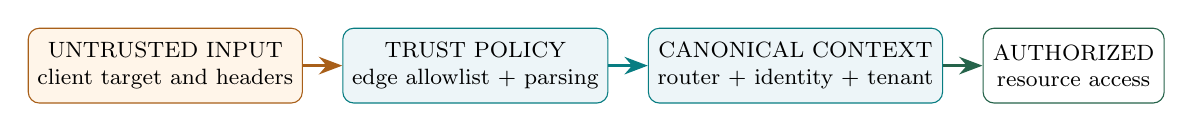
\begin{tikzpicture}[font=\footnotesize,node distance=5mm]
\node[draw=orange,fill=softorange,rounded corners,minimum width=3.1cm,minimum height=0.95cm,align=center] (a) {UNTRUSTED INPUT\\client target and headers};
\node[draw=teal,fill=pale,rounded corners,right=of a,minimum width=3.1cm,minimum height=0.95cm,align=center] (b) {TRUST POLICY\\edge allowlist + parsing};
\node[draw=teal,fill=pale,rounded corners,right=of b,minimum width=3.1cm,minimum height=0.95cm,align=center] (c) {CANONICAL CONTEXT\\router + identity + tenant};
\node[draw=forest,fill=white,rounded corners,right=of c,minimum width=2.3cm,minimum height=0.95cm,align=center] (d) {AUTHORIZED\\resource access};
\draw[very thick,-{Stealth},orange] (a)--(b);
\draw[very thick,-{Stealth},teal] (b)--(c);
\draw[very thick,-{Stealth},forest] (c)--(d);
\end{tikzpicture}
\caption{Request metadata becomes security-relevant only after explicit boundary validation.}
\end{figure}

\subsection{Threat-to-control matrix}
\footnotesize
\begin{longtable}{P{0.23\linewidth}P{0.20\linewidth}P{0.47\linewidth}}
\toprule
\textbf{Threat / weakness} & \textbf{Affected metadata} & \textbf{Primary controls and validation}\\\midrule\endfirsthead
\toprule\textbf{Threat / weakness} & \textbf{Affected metadata} & \textbf{Primary controls and validation}\\\midrule\endhead
Path traversal (CWE-22) & Decoded / translated path, user-supplied filenames & Do not splice URL path into disk paths. Resolve under an immutable configured root; enforce containment and authorization; deny symlink escape where appropriate.\\
Inconsistent request interpretation (CWE-444) & Raw target, decoded path, request framing & Align proxy/origin normalization; reject ambiguous encodings and malformed framing; fuzz edge-to-app consistency.\\
Host-header injection & \code{Host}, \code{:authority}, forwarded host & Reject unknown hosts; configure public origin and allowed hosts; do not construct password-reset or redirect URLs using arbitrary host claims.\\
Proxy-header spoofing & Forwarded-for/proto/host & Accept metadata only from known proxies; overwrite client-supplied forwarding headers at the ingress; limit chain length / hops.\\
Open redirect (CWE-601) & \code{returnUrl}, \code{next}, host & Use relative destinations or strict absolute-URL origin allowlists; validate before redirecting.\\
Sensitive query leakage (CWE-598) & Raw query, full URL, \code{Referer} & Never put access tokens or secrets in query; redact logs/traces; prefer proper authentication headers, short-lived purpose-bound credentials.\\
SSRF (CWE-918) & Host, URL / callback parameters & Enforce destinations and schemes, DNS/IP policy, and egress policy for server-side fetches; avoid user-defined callback hosts.\\
Response splitting (CWE-113) & Untrusted header-bound values & Use framework header APIs; reject CR/LF and unsafe control characters; do not assemble HTTP header lines manually.\\
Access-control bypass (CWE-20 / related) & Route capture, tenant identifier, decoded path & Validate normalized route ID, apply object authorization, and keep one source of truth for routing across middleware.\\
Information exposure (CWE-200) & Debug metadata, environment values, IPs & Protect/remove inspection endpoints; mask tokens, internal topology, filesystem details and private identifiers.\\
\bottomrule
\end{longtable}
\normalsize
\emph{CWE mappings are representative categories, not claims that a particular library or example contains a vulnerability.} The precise weakness classification depends on the exploitable behavior and the application context.

\subsection{Canonicalization and path containment}
\begin{enumerate}
\item Identify the representation received from the ingress: original raw target if supplied, then server-decoded path, then router-selected resource.
\item Specify encoding policies: reject malformed percent triplets, disallowed separators, NUL/control characters, dot-segment ambiguity, and double-encoded traversal as relevant to the endpoint.
\item Avoid ad-hoc successive decoding. Decode components only at the intended boundary, then validate the resulting canonical representation. Differences in proxy and app behavior deserve dedicated tests.
\item For file access, combine an application-owned storage root with a normalized relative reference, enforce containment, and check authorization. For attacker-writable directories, race-resistant file-opening and symlink policies are also required.
\item Keep the security decision attached to the final resource identifier, not to an earlier, differently encoded string.
\end{enumerate}
\begin{lstlisting}[language=Python,caption={Illustration: validated path containment for a read-only repository}]
from pathlib import Path

ROOT = Path('/srv/public-assets').resolve(strict=True)

def resolve_asset(relative_name: str) -> Path:
    # Reject absolute paths; path decoding was handled upstream.
    candidate = Path(relative_name)
    if candidate.is_absolute() or '\x00' in relative_name:
        raise ValueError('invalid asset name')
    resolved = (ROOT / candidate).resolve(strict=True)
    if not resolved.is_relative_to(ROOT):
        raise ValueError('outside asset root')
    return resolved
\end{lstlisting}
\textbf{Boundary of this example:} \code{Path.resolve()} plus containment is an illustrative path validation pattern, not a complete symlink-race defense. Restrict directory write permissions, consider descriptor-relative OS APIs for adversarial filesystems, and authorize each resolved asset before reading. Python 3.9+ provides \code{Path.is\_relative\_to()}.

\subsection{Trusted reverse-proxy configuration}
RFC 7239 defines a standardized \code{Forwarded} field, while many deployments use the nonstandard but widespread \code{X-Forwarded-*} family. They are statements placed in HTTP fields and \emph{not} automatically truthful.\refs{18}
\begin{keybox}
\textbf{Deployment checklist}\par
\begin{enumerate}
\item Identify every edge/gateway hop and which hop terminates TLS.
\item Restrict direct origin access to expected proxy networks or authenticated service identities.
\item At the trusted entry point, \emph{remove and regenerate} externally supplied forwarding fields according to policy.
\item Configure the application to accept forwarded information only from known peers; set hop count/chain behavior.
\item Define whether external mount prefix and host are forwarded or configured statically.
\item Constrain public hostnames to an allowlist. Prefer a configured canonical origin for security-sensitive emails and redirects.
\item Verify direct-access, forged-header, multi-hop, and scheme mismatch cases.
\end{enumerate}
\end{keybox}

\subsection{Secure URL construction and redirects}
\begin{lstlisting}[language=JavaScript,caption={Express: configure the canonical public origin rather than trusting Host}]
const PUBLIC_ORIGIN = new URL('https://accounts.example.test');

app.get('/reset-link', (req, res) => {
  // Example only: authentication, authorization, and a secure reset
  // token generator must be implemented separately.
  const link = new URL('/account/reset', PUBLIC_ORIGIN);
  res.json({resetPage: link.toString()});
});
\end{lstlisting}
Do not copy a client-supplied \code{redirect}, \code{next}, \code{Host}, or \code{X-Forwarded-Host} directly into a security-sensitive absolute URL. \code{Origin} or \code{Referer} may contribute to a browser security check, but neither replaces authentication, CSRF protections, or endpoint authorization.

\subsection{Safe logging and privacy}
\begin{tabularx}{\linewidth}{P{0.29\linewidth}Y}
\toprule\textbf{Preferred log field} & \textbf{Policy}\\\midrule
Route template (e.g., \code{/orders/\{id\}}) & Prefer over raw URL for high-cardinality and personal-data reduction.\\
Validated request ID / trace ID & Format/length validate, generate internally if missing; never use as proof of identity.\\
Normalized method, status, duration & Safe observability baseline, with careful correlation to authenticated user if necessary.\\
Query string and path identifiers & Usually mask, hash, or omit sensitive terms; define retention and access.\\
Headers and cookies & Allowlist safe fields; never log credentials, cookies, bearer tokens, or application secrets.\\
\bottomrule
\end{tabularx}

\section{Reference test suite and verification workflow}
\subsection{Baseline commands}
Bring up a \emph{single} diagnostic implementation on \code{127.0.0.1:8000}; then adapt the path to the framework's example mapping (\code{/inspect}, \code{/inspect/}, etc.). The commands below exercise the local endpoint without depending on public infrastructure.
\begin{lstlisting}[language=bash,caption={cURL smoke tests: local development instance}]
# Duplicate query parameters, escaping and query order
curl -i --path-as-is \
 'http://127.0.0.1:8000/inspect/a%2Fb?tag=red&tag=blue&next=%2Fcart'

# Empty query versus query absent: interface-dependent distinction
curl -i 'http://127.0.0.1:8000/inspect/?'
curl -i 'http://127.0.0.1:8000/inspect/'

# Dot segments; compare proxy, server, and router behavior
curl -i --path-as-is \
 'http://127.0.0.1:8000/inspect/a/../b?x=1'

# Claimed authority: NEVER treat this as trusted by itself
curl -i -H 'Host: untrusted.example.test' \
 'http://127.0.0.1:8000/inspect/'

# Forwarded fields can be forged when edge policy is absent
curl -i -H 'X-Forwarded-Proto: https' \
        -H 'X-Forwarded-For: 203.0.113.25' \
 'http://127.0.0.1:8000/inspect/'
\end{lstlisting}
The \code{--path-as-is} flag prevents cURL itself from normalizing dot-segments in some requests. Not every stack accepts every malformed or unusual request; a rejection can be the correct security outcome. Use the tests to record the effective behavior, not to force identical outputs across different abstractions.

\subsection{Cross-layer test matrix}
\footnotesize
\begin{longtable}{P{0.24\linewidth}P{0.32\linewidth}P{0.34\linewidth}}
\toprule\textbf{Case} & \textbf{Probe} & \textbf{Expected invariant}\\\midrule\endfirsthead
\toprule\textbf{Case} & \textbf{Probe} & \textbf{Expected invariant}\\\midrule\endhead
Ordinary URL & \code{/items/42?view=full} & Router resolves intended resource; query is distinct from path.\\
Repeated query key & \code{tag=a\&tag=b} & Explicit first/last/multi/reject policy, consistent at edge and app.\\
Encoded slash & \code{/a\%2Fb} & Deliberate handling with no unexpected route/authorization bypass.\\
Dot segments & \code{/a/../b} & Edge and app have compatible canonicalization and deny policies.\\
Double encoding & \code{\%252e\%252e\%252f} & No second-decode authorization bypass.\\
Malformed escape & \code{/a\%ZZ} & Reject or defined handling; no inconsistent reinterpretation downstream.\\
Empty / missing query & \code{/p?} vs \code{/p} & Product contract defined if distinction matters; Go has \code{ForceQuery}.\\
Unicode paths & UTF-8 encoded non-ASCII name & Explicit character/normalization policy and test coverage.\\
Conflicting hosts & \code{Host} vs forwarded host or \code{:authority} & Consistent rejection/allowlist policy; no host-based privilege change.\\
Untrusted forwarded chain & Forged \code{X-Forwarded-For} & Peer attribution changes only under trusted proxy rules.\\
TLS offload & External HTTPS, internal HTTP & Correct secure URL generation only under trusted scheme policy.\\
Mounted app & External \code{/store/api} vs internal \code{/api} & Prefix handled once; route and public links remain correct.\\
Path-parameter collision & \code{/tenant/A/orders/B} & Authorization binds to validated tenant/resource ID rather than original path string.\\
Long URL / repeated inputs & Oversized target, many parameters & Request-size limits enforced; parsing latency/memory bounded.\\
HTTP framing ambiguity & Invalid duplicate framing headers & Rejected at gateway or origin per configured protocol policy.\\
Sensitive query & \code{?token=example-secret} & Secret absent from application logs/traces and downstream referrals.\\
\bottomrule
\end{longtable}
\normalsize

\subsection{Metadata contract for a service}
Use this mini-template in an architecture decision record, API security review, or ingestion contract.
\begin{table}[h!]
\centering\small
\begin{tabularx}{\linewidth}{P{0.28\linewidth}Y}
\toprule\textbf{Decision} & \textbf{Document explicitly}\\\midrule
Authoritative URI path & Which layer parses, normalizes, rejects, and routes.\\
Query cardinality & Per-key duplicate rules, maximum key/value length, allowed formats.\\
External origin & Fixed scheme/host/port; allowed hostnames; redirects and reset-link policy.\\
Ingress trust & Trusted hops, header rewrite behavior, direct-origin controls.\\
URL encoding & Percent decoding, UTF-8, encoded slash policy, Unicode normalization if applicable.\\
Identity / authorization & Authenticated principal and resource IDs; enforcement point after route resolution.\\
Diagnostics & Fields exported, redaction controls, access, retention, monitoring.\\
Regression ownership & Tests run at unit, integration, edge-to-origin, and preproduction layers.\\
\bottomrule
\end{tabularx}
\end{table}

\section{Practical selection guide}
\begin{longtable}{P{0.32\linewidth}P{0.58\linewidth}}
\toprule\textbf{Task} & \textbf{Recommended first interface}\\\midrule\endfirsthead
\toprule\textbf{Task} & \textbf{Recommended first interface}\\\midrule\endhead
Route-specific business logic & Jakarta servlet mapping / Jakarta REST route; ASP.NET Core route values; PHP router; Python framework route; Express route; Go mux route.\\
Raw target diagnostics & Java \code{getRequestURI()+getQueryString()} (not guaranteed byte-original); ASP.NET Core raw-target server feature where available; PHP \code{REQUEST\_URI}; ASGI \code{raw\_path}+\code{query\_string}; Node \code{req.url}; Go \code{RequestURI}.\\
Normal query parsing & Java \code{getParameterValues()}; ASP.NET Core \code{Request.Query}; PHP \code{\$\_GET} with explicit duplicate contract; Python framework parser / \code{parse\_qs}; Node \code{URLSearchParams}; Go \code{URL.Query()}.\\
Mount prefix & Java \code{getContextPath()} + servlet mapping; ASP.NET Core \code{PathBase}; PHP web-server/router configuration; WSGI \code{SCRIPT\_NAME}; ASGI \code{root\_path}; Express \code{baseUrl}; Go explicit mux/proxy configuration.\\
Public absolute URL & A separately configured canonical public origin, optionally combined with framework-aware path generation.\\
Client identity & Auth framework validated principal; do not confuse with IP address, host, forwarded metadata, or tracing IDs.\\
File-system asset & Storage/service abstraction with safe path resolution and authorization; \emph{not} \code{PATH\_TRANSLATED}.\\
\bottomrule
\end{longtable}

\section{Standards and vendor documentation}
These are primary references used to inform this guide. The interface names and protocol distinctions should be validated against the exact runtime release, ingress configuration, and container/server implementation deployed by the organization. Retrieved/checked October 2026.
\begin{enumerate}[label={[\arabic*]},leftmargin=2.1em,itemsep=6pt]
\item \textbf{RFC 3986 --- URI Generic Syntax.} \url{https://www.rfc-editor.org/rfc/rfc3986.html}. URI components, escaping, dot-segments and normalization.
\item \textbf{RFC 9110 --- HTTP Semantics.} \url{https://www.rfc-editor.org/rfc/rfc9110.html}. Target URI, authority, method semantics and HTTP fields.
\item \textbf{RFC 9112 --- HTTP/1.1.} \url{https://www.rfc-editor.org/rfc/rfc9112.html}. Request-target forms, Host handling and framing.
\item \textbf{RFC 9113 --- HTTP/2.} \url{https://www.rfc-editor.org/rfc/rfc9113.html}. Request control pseudo-headers and authority handling.
\item \textbf{RFC 9114 --- HTTP/3.} \url{https://www.rfc-editor.org/rfc/rfc9114.html}. Request control pseudo-headers over HTTP/3.
\item \textbf{RFC 3875 --- CGI/1.1.} \url{https://www.rfc-editor.org/rfc/rfc3875.html}. \code{PATH\_INFO}, \code{PATH\_TRANSLATED}, \code{QUERY\_STRING}, \code{SCRIPT\_NAME}.
\item \textbf{Jakarta Servlet 6.1 API.} \url{https://jakarta.ee/specifications/servlet/6.1/apidocs/jakarta.servlet/jakarta/servlet/http/httpservletrequest}. \code{HttpServletRequest} contract.
\item \textbf{ASP.NET Core HttpRequest API.} \url{https://learn.microsoft.com/en-us/dotnet/api/microsoft.aspnetcore.http.httprequest}. Request path, query, scheme, host and route values.
\item \textbf{PHP manual --- \code{\$\_SERVER}.} \url{https://www.php.net/manual/en/reserved.variables.server.php}. Server and request variables.
\item \textbf{PEP 3333 --- WSGI for Python 3.} \url{https://peps.python.org/pep-3333/}. WSGI environment and URL reconstruction.
\item \textbf{ASGI HTTP/WebSocket protocol spec.} \url{https://asgi.readthedocs.io/en/latest/specs/www.html}. Request scope and raw path/query metadata.
\item \textbf{Node.js HTTP API.} \url{https://nodejs.org/api/http.html}. \code{IncomingMessage} and duplicate header handling.
\item \textbf{Express 5.x API.} \url{https://expressjs.com/en/5x/api.html} and \url{https://expressjs.com/en/5x/api/application/}. Routing, query parsing and \code{trust proxy}.
\item \textbf{Go standard library \code{net/http}.} \url{https://pkg.go.dev/net/http}. HTTP request fields and routing.
\item \textbf{ASP.NET Core proxy/load balancer guidance.} \url{https://learn.microsoft.com/en-us/aspnet/core/host-and-deploy/proxy-load-balancer}. Known proxies and forwarded headers.
\item \textbf{Express trust-proxy guide.} \url{https://expressjs.com/en/guide/behind-proxies.html}. Trust configuration and forwarded identity.
\item \textbf{Go standard library \code{net/url}.} \url{https://pkg.go.dev/net/url}. Decoding, \code{RawPath}, \code{EscapedPath()}, raw query and \code{ForceQuery}.
\item \textbf{RFC 7239 --- Forwarded HTTP Extension.} \url{https://www.rfc-editor.org/rfc/rfc7239.html}. Standardized (but not inherently authenticated) proxy metadata.
\end{enumerate}

\clearpage
\section*{Final engineering checklist}
\addcontentsline{toc}{section}{Final engineering checklist}
\begin{keybox}
\begin{itemize}[label=$\square$,leftmargin=2em,itemsep=6pt]
\item The request target, raw query, parsed query, and route captures are individually understood and tested.
\item Encoded slash, dot-segment, malformed escape, repeated parameter, and empty-query behavior are specified.
\item Edge and origin parsing, URI rewriting, and tenant/resource authorization are consistent.
\item Host and forwarded metadata are accepted only under verified policies; public origin is allowlisted/configured.
\item Diagnostics cannot leak credentials, cookies, filesystem paths, request bodies, or sensitive URLs.
\item \code{PATH\_TRANSLATED} is not relied on as a universal route or secure filesystem reference.
\item Functional tests are repeated through the \emph{production-like ingress chain}, not just against a local development port.
\item Changes in framework major version, web server, reverse proxy, or URI-routing policy trigger regression tests.
\end{itemize}
\end{keybox}
\vspace{0.28in}
\begin{center}
{\large\bfseries\color{navy}Correct metadata interpretation starts with a documented trust boundary.}\\[7pt]
{\color{graytext}Identify the representation. Validate the source. Bind authorization to the resolved resource.}
\end{center}
\end{document}
